\documentclass[,UTF8,titlepage]{ctexart}
\usepackage{booktabs,multirow,subfig}
\usepackage{graphicx}
\usepackage{amsmath,amsthm}
\usepackage{xcolor}

\usepackage{tikz}

\usepackage{hyperref}
\hypersetup{hidelinks}
\usepackage{indentfirst}
\setlength{\parindent}{2em}


\title{\LaTeX{} \emph{Primer} \thanks{110分钟\LaTeX{}入门}}
\author{田阳 \thanks{Yeungtien@gmail.com}
\and Knuth, Donald Ervin \thanks{\LaTeX{} author}}
\date{\today}
\linespread{1.5}
\pagestyle{plain}
\bibliographystyle{plain}

\begin{document}
\maketitle
\abstract{这是对\LaTeX{} 简短的复现。}
\newpage
\thispagestyle{empty}
\tableofcontents
\newpage
\setcounter{page}{1}
\section{Just for Trying} \label{one}
\begin{center}
    ``Hello,\emph{world}''\footnote{这是一个脚注} \par
    \marginpar{\footnotesize 这是一个边注} 
\end{center}
\subsection{引用}
\begin{flushright}
    我尝试引用章节 \ref{one} 以及它的页码 \pageref{one},并把这句话右对齐 
\end{flushright}
鲁迅说过:\par
\begin{quotation}
    我没有这样说过 
\end{quotation}
\subsection{列表}
\begin{enumerate}
\item 这是有序列表第一项
    \begin{enumerate}
       \item 这是有序列表的子列表 \label{sublist}
       \item[*] 加个star会怎样呢 
    \end{enumerate}
\item 引用子列表(\ref{sublist})
\end{enumerate}
\begin{itemize}
    \item 这是无序列表第一项
    \begin{itemize}
        \item 这是无序列表子列表
        \item[+] 加个plus会怎样呢
    \end{itemize}
    \item description环境
    \begin{description}
        \item[enumerate] 有序列表
        \item[itemize] 无序列表
    \end{description}
\end{itemize}
%我想改无序列表的符号\renewcommand{\labelitemi}{\ddag}
%我想改有序列表的符号\renewcommand{\labelenumi}{\ddag}
\subsection{代码}
\begin{verbatim}
for i in range(1024):
    print(`Hello,world')
\end{verbatim}
\verb|这表示简短的代码或关键词|
\subsection{表格}
\verb|三线表|
\begin{tabular}{cccc}
 \toprule
 \multirow{2}{*}{Item} & \multicolumn{3}{c}{number}\\% 用于合并单元格
 \cmidrule{2-4}
    & 1 & 2 & 3 \\
\midrule
Alphabeta & A & B & C \\ \cline{2-3}
Number & 1 & 2 & 3 \\[6pt]
\bottomrule
\end{tabular}
\subsection{盒子}
\setlength{\fboxrule}{1.6pt}
\setlength{\fboxsep}{1em}
\framebox[10em][r]{这是个盒子}
\subsection{浮动体初探}
\begin{figure}[h]
    \centering
    \subfloat{
    \begin{minipage}[t]{0.3\textwidth} 
    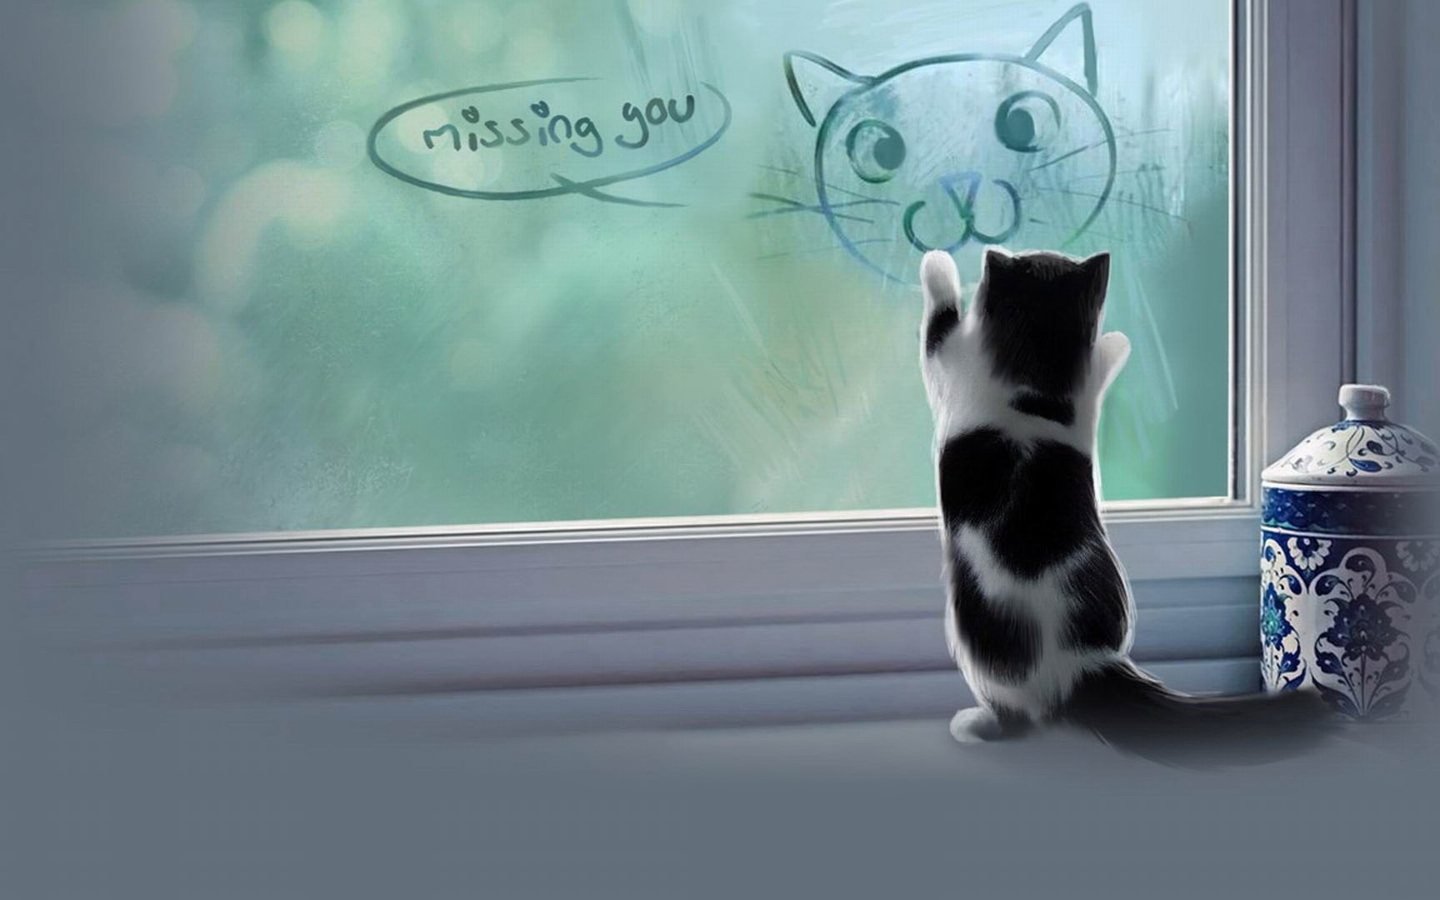
\includegraphics[width=.8\textwidth]{cat.jpg}
    \caption{小猫猫}
    \label{fig:cutecat}
    \end{minipage}
    }
    \quad
    \subfloat{
    \begin{minipage}[t]{0.3\textwidth} 
        \includegraphics[width=.8\textwidth]{sugar.jpg}
        \caption{小糖糖}
        \label{fig:cutesugar}
    \end{minipage}
    }
    \caption{并排图表}
\end{figure}
\section{进阶公式}
\subsection{初级}
\subsection{一些字母及公式}
\begin{equation}
    E=hv \tag{普朗克公式}\label{eq1} 
\end{equation}
我引用\eqref{eq1}来演示 \\
$ E'(v) \leftrightarrow 粒子 \qquad \text{ \textbf{能量}是离散的粒子 }  $ \\
Pascal's rule: \\
\[
    \binom{n}{k} =\binom{n-1}{k} + =\binom{n-1}{k-1}
\] \\
一些关系符$\neq \geq \leq \approx \propto  \stackrel{*}{\sim} $
一些运算符$\times \div \cdot \pm \nabla \partial$
一些巨算符$\sum\limits_{i=1}^n \quad \sum\nolimits_{i=1}^n \quad \int_0^{\frac{\pi}{2}} \quad \prod_\epsilon \quad $
还有\[
    \sum_{\substack{0 \le i \le n \\
    j \in R}}
    p(i,j)=Q(n)\\
    \bar{x} \quad \vec{x_0} \quad \hat{\mathbf{e}}
\]\\
$\underbrace{\overbrace{(a+b+c)}^6\cdot\overbrace{(c\times d)}^7}_\text{这是下括号}=42$\\
以及定界符:$1+\left(\frac{\pi}{\epsilon}\right)^n \quad 
\left.\frac{\partial f}{\partial x}\right |_t=0$ \par
\begin{align}
    \text{等号对齐}\\  \notag
    a &= b+c \\  
    d &= e+f \\
\end{align}

\begin{gather}
    \text{罗列公式}\\ \notag
    a = b+c \\  
    d = e+f \\
\end{gather}
\begin{equation}
    \text{公用编号}\\
    \begin{aligned}
    a &= b+c \\  
    d &= e+f \\ 
    \end{aligned}
\end{equation}

\[|\textbf{x}|=\left\{
    \begin{array}{rl}
       -x  & if \quad x < 0,\\
       0 & if \quad  x = 0, \\
       x & if \qquad x >0 \\ 
    \end{array}
    \right.
\]\\
% same as:begin{cases}
\subsection{定理环境}
%\newtheorem{环境名}{定理}[所属章节]
\newtheorem{new}{定理}[subsection]
\begin{new} \label{ref:thm1}
    这是\textbf{定理1}
\end{new}
\begin{new}[定理名]
    这是定理2,引用\ref{ref:thm1}
\end{new}
\begin{proof}
我用此来证明:
\[
    \textbf{此言非虚} \qedhere
\]    
\end{proof}
\section{特色工具}
\subsection{参考文献}
{\small 以下是 {\large 参考文献}}\\
% 这是参考自\cite[page 1024]{reference1}的句子
% \begin{thebibliography}{99}
%     \bibitem{reference1} Tien:\emph{Yeung} ,2019
% \end{thebibliography}
这是参考自\cite[page 1024]{book1}的句子
\bibliography{book}
\subsection{颜色}
{\color[gray]{0.8} 灰色}
{\color[rgb]{0,1,1} 青色}
{\color{yellow} 黄色}
\textcolor{red}{红色}
\colorbox{green}{绿色的盒子}
\fcolorbox{black}{magenta}{黑色边框,玫红背景}
\subsection{超链接}
\url{www.baidu.com} \\
\href{www.baidu.com}{F*CK}
\section{绘图}
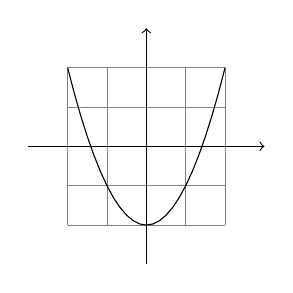
\begin{tikzpicture}
\draw[help lines,step=0.5]
    (-1,-1)grid(1,1);
\draw[->] (-1.5,0)--(1.5,0);
\draw[->] (0,-1.5)--(0,1.5);
\draw[domain=-1:1]
    plot(\x,{\x*\x*2 -1});
\end{tikzpicture}
\end{document}


